% === X. LAMPIRAN ===
\clearpage
\secbox{X.}{LAMPIRAN}

\lampiranhead{1. Business Process / Workflow}
\begin{figure}[H]
    \centering
    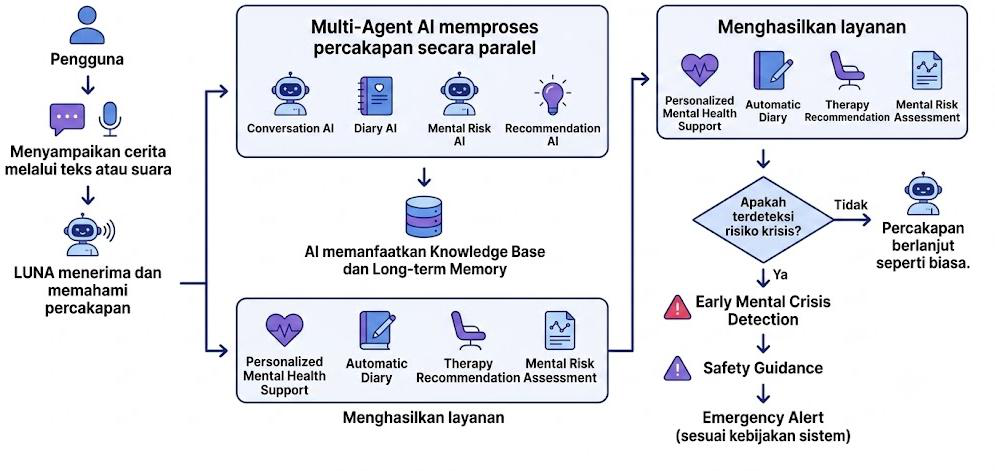
\includegraphics[width=0.92\textwidth]{images/lampiran/fig6_business_process.png}
    \caption{Proses Bisnis LUNA}
\end{figure}

\lampiranhead{2. Use case Diagram}
\begin{figure}[H]
    \centering
    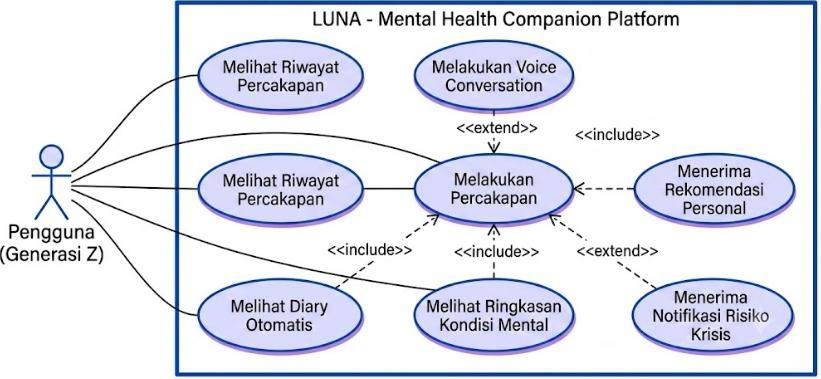
\includegraphics[width=0.88\textwidth]{images/lampiran/fig7_usecase.png}
    \caption{Use Case Diagram}
\end{figure}

\lampiranhead{3. Arsitektur Multi-Agent AI}
\begin{figure}[H]
    \centering
    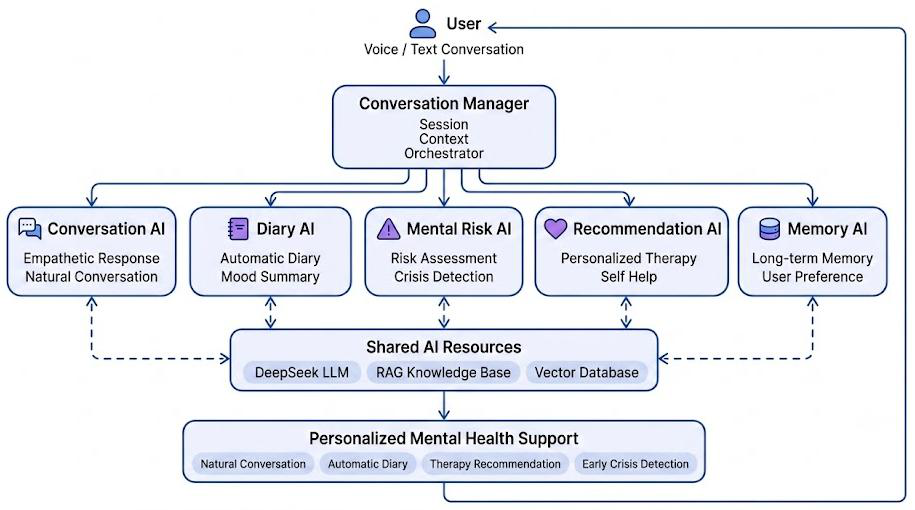
\includegraphics[width=0.92\textwidth]{images/lampiran/fig8_multiagent_architecture.png}
    \caption{Arsitektur Multi-Agent AI}
\end{figure}

\lampiranhead{4. Mockup Interface Application}

\subsubsecstyle{a. Register}
\begin{figure}[H]
    \centering
    \begin{tikzpicture}
        \node[
            draw=TealAccent,
            fill=white,
            line width=0.8pt,
            rounded corners=6pt,
            inner sep=2pt
        ] {
            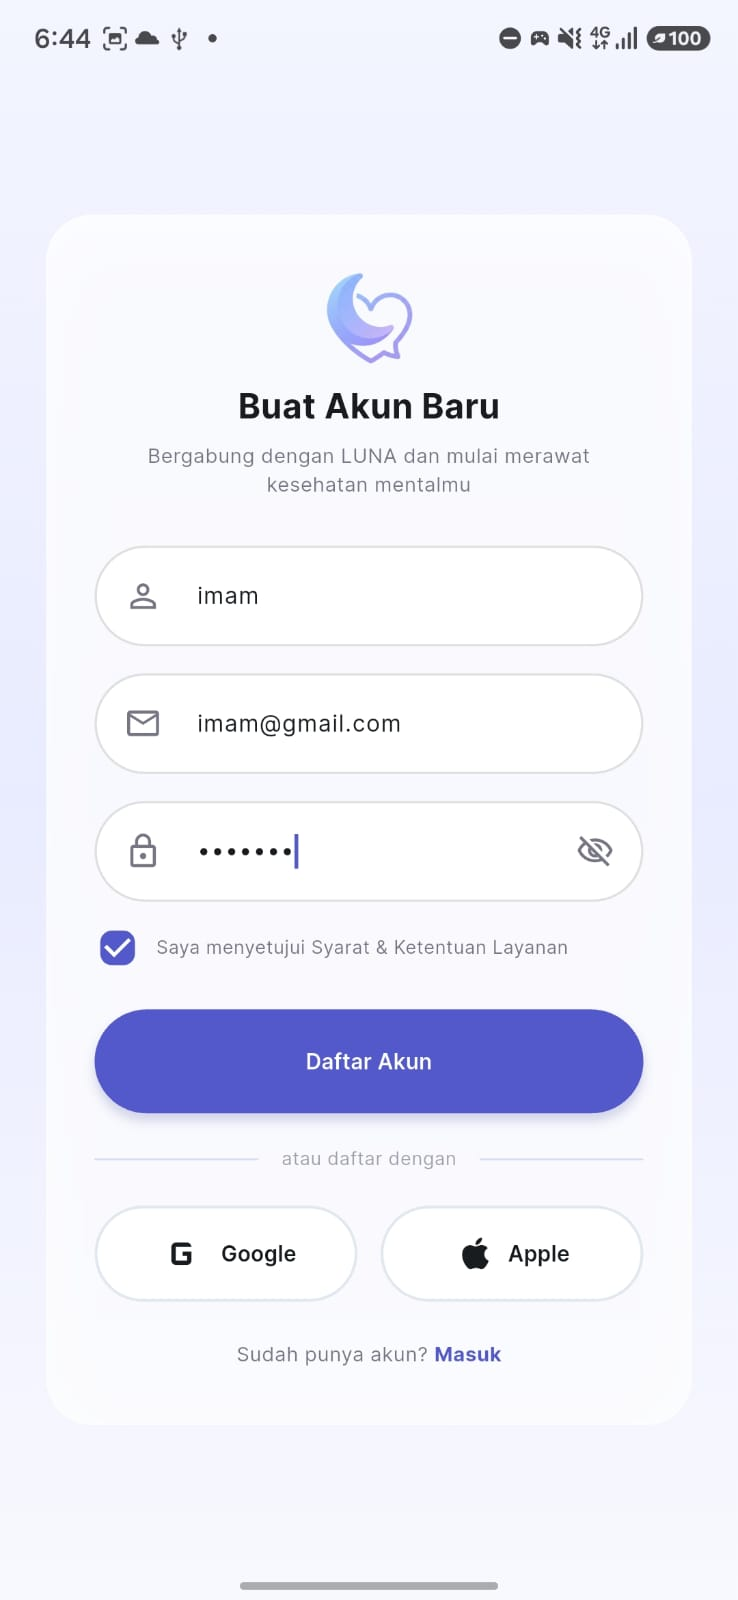
\includegraphics[height=5.8cm,keepaspectratio]{images/prototype/auth_signup.jpeg}
        };
    \end{tikzpicture}
    \caption{Register}
\end{figure}

\subsubsecstyle{b. Login}
\begin{figure}[H]
    \centering
    \begin{tikzpicture}
        \node[
            draw=TealAccent,
            fill=white,
            line width=0.8pt,
            rounded corners=6pt,
            inner sep=2pt
        ] {
            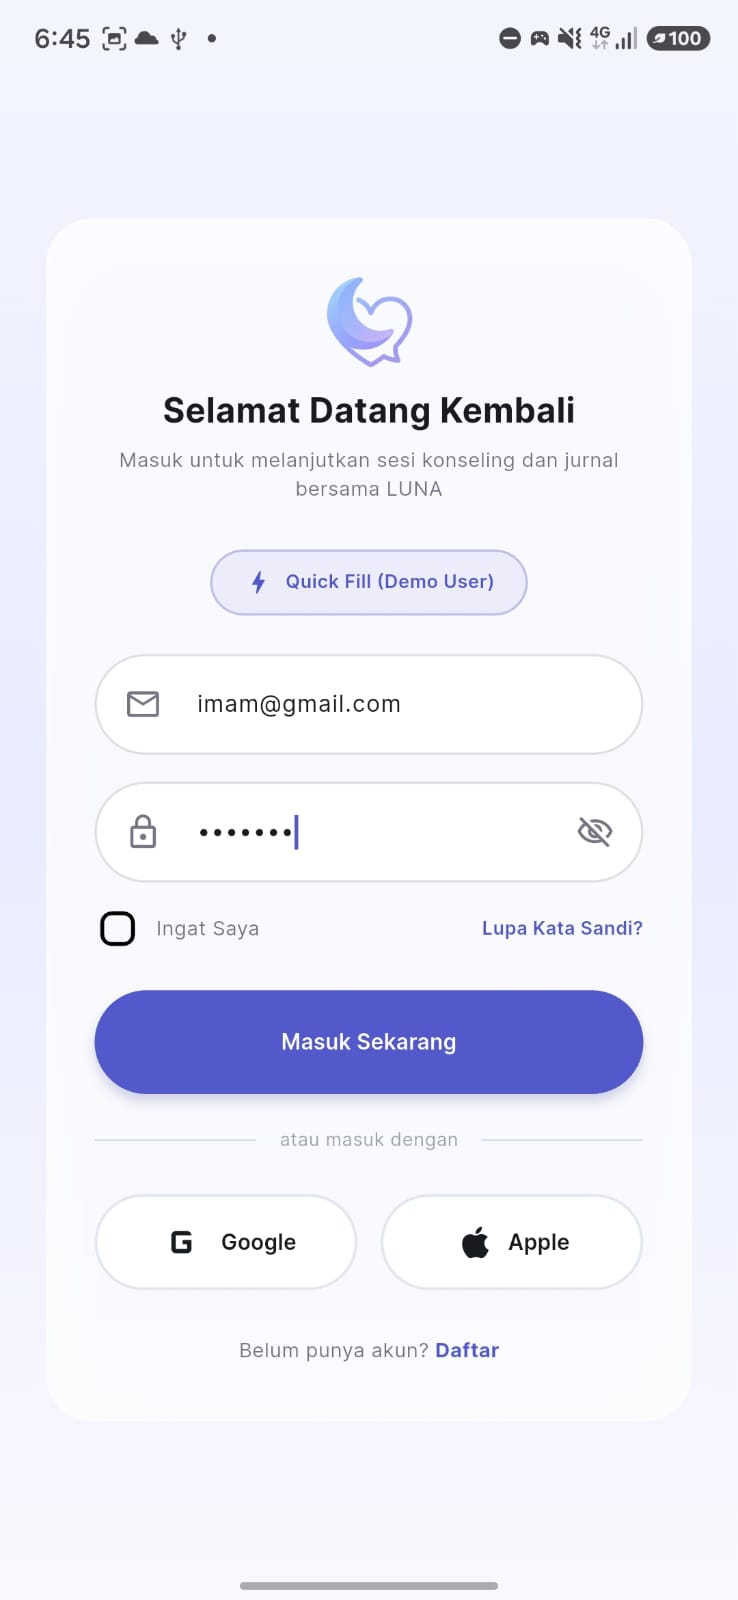
\includegraphics[height=5.8cm,keepaspectratio]{images/prototype/auth_signin.jpeg}
        };
    \end{tikzpicture}
    \caption{Login}
\end{figure}

\subsubsecstyle{c. Onboarding}
\begin{figure}[H]
    \centering
    \begin{tikzpicture}
        \node[
            draw=TealAccent,
            fill=white,
            line width=0.8pt,
            rounded corners=6pt,
            inner sep=2pt
        ] {
            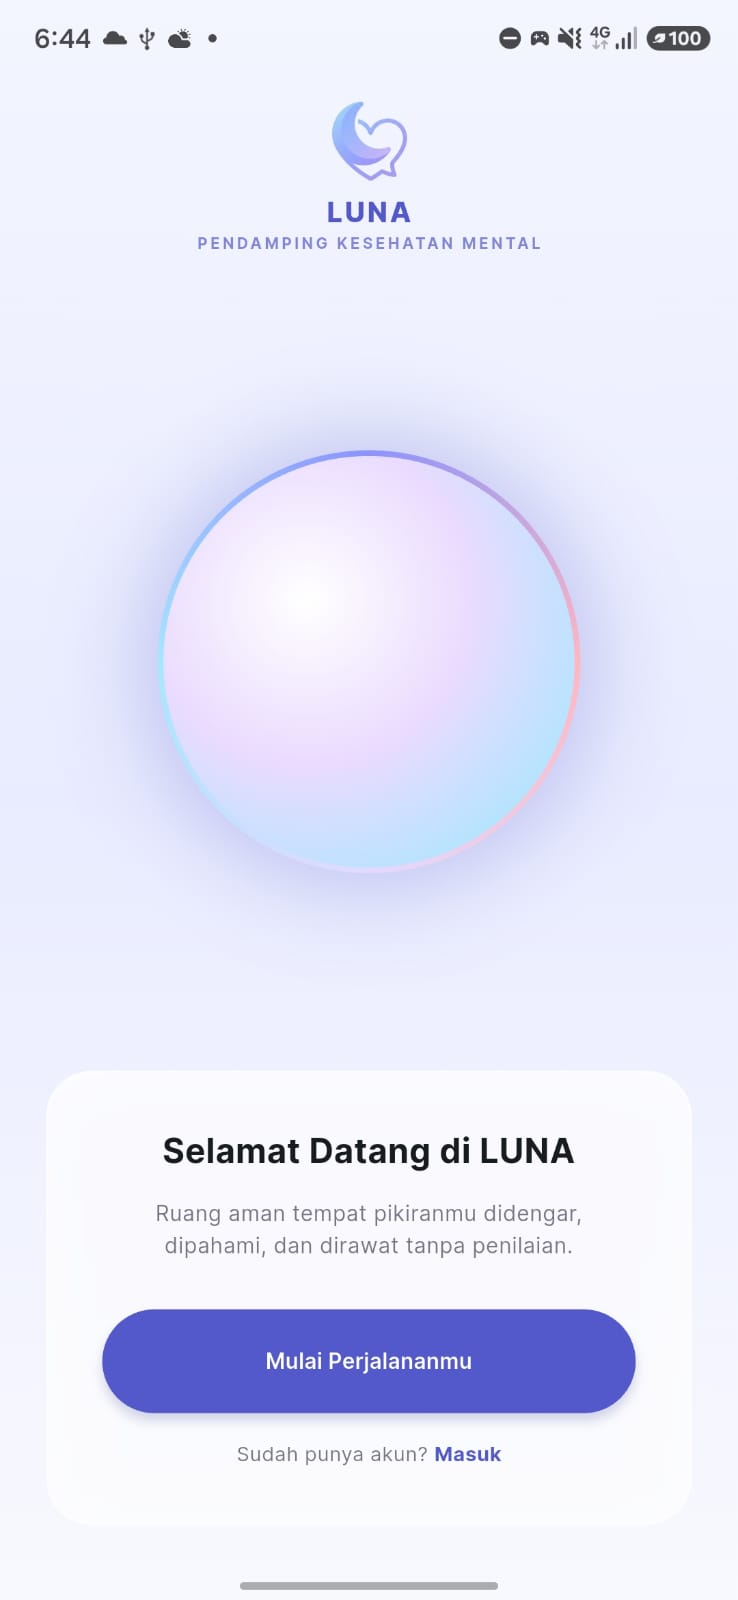
\includegraphics[height=5.8cm,keepaspectratio]{images/prototype/auth_firstscreen.jpeg}
        };
    \end{tikzpicture}
    \caption{Onboarding}
\end{figure}

\subsubsecstyle{d. Home}
\begin{figure}[H]
    \centering
    \begin{tikzpicture}
        \node[
            draw=TealAccent,
            fill=white,
            line width=0.8pt,
            rounded corners=6pt,
            inner sep=2pt
        ] {
            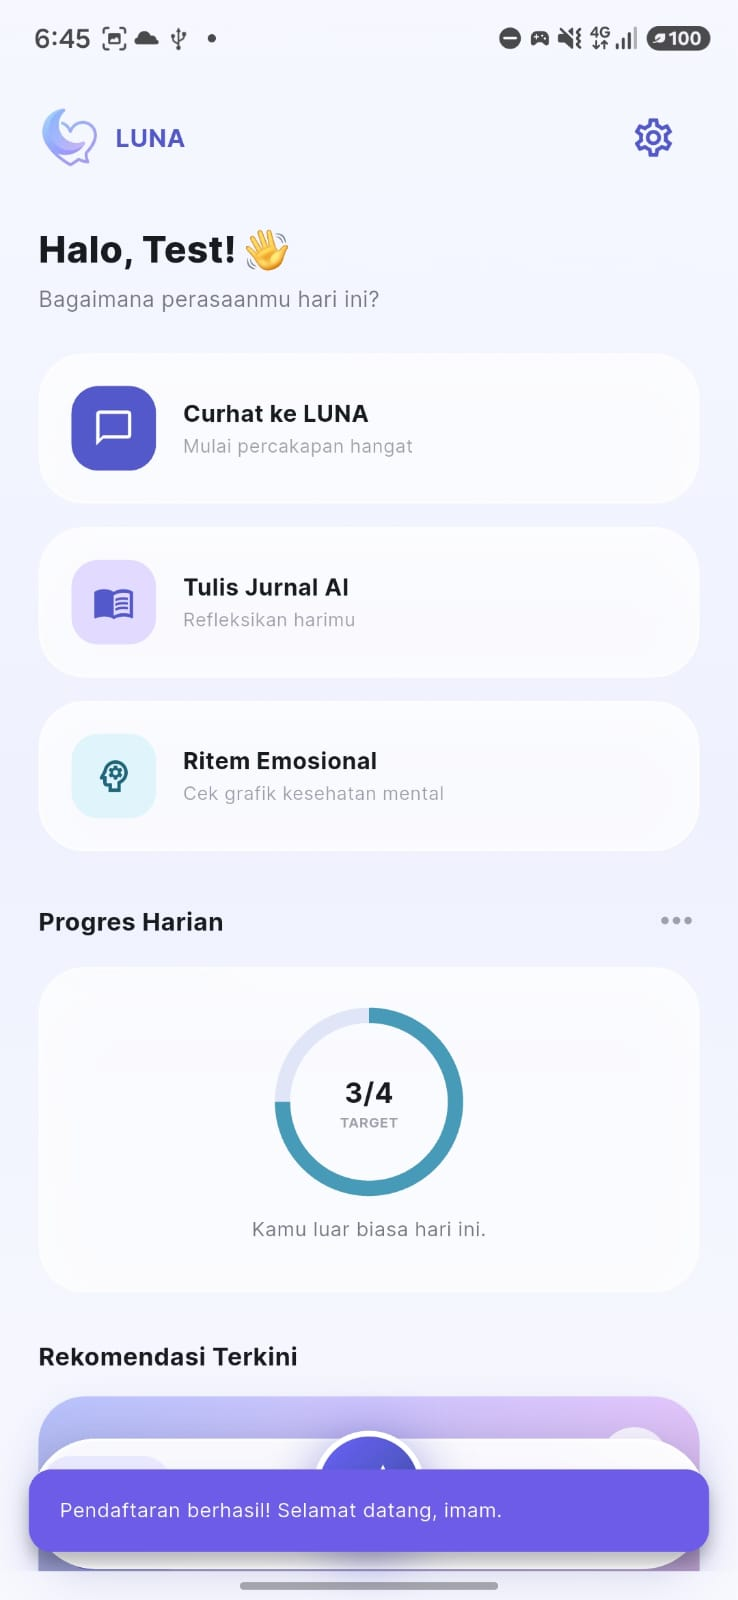
\includegraphics[height=5.8cm,keepaspectratio]{images/prototype/auth_home.jpeg}
        };
    \end{tikzpicture}
    \caption{Home}
\end{figure}

\subsubsecstyle{e. AI Conversation}
\begin{figure}[H]
    \centering
    \begin{minipage}[b]{0.45\textwidth}
        \centering
        \begin{tikzpicture}
            \node[
                draw=TealAccent,
                fill=white,
                line width=0.8pt,
                rounded corners=6pt,
                inner sep=2pt
            ] {
                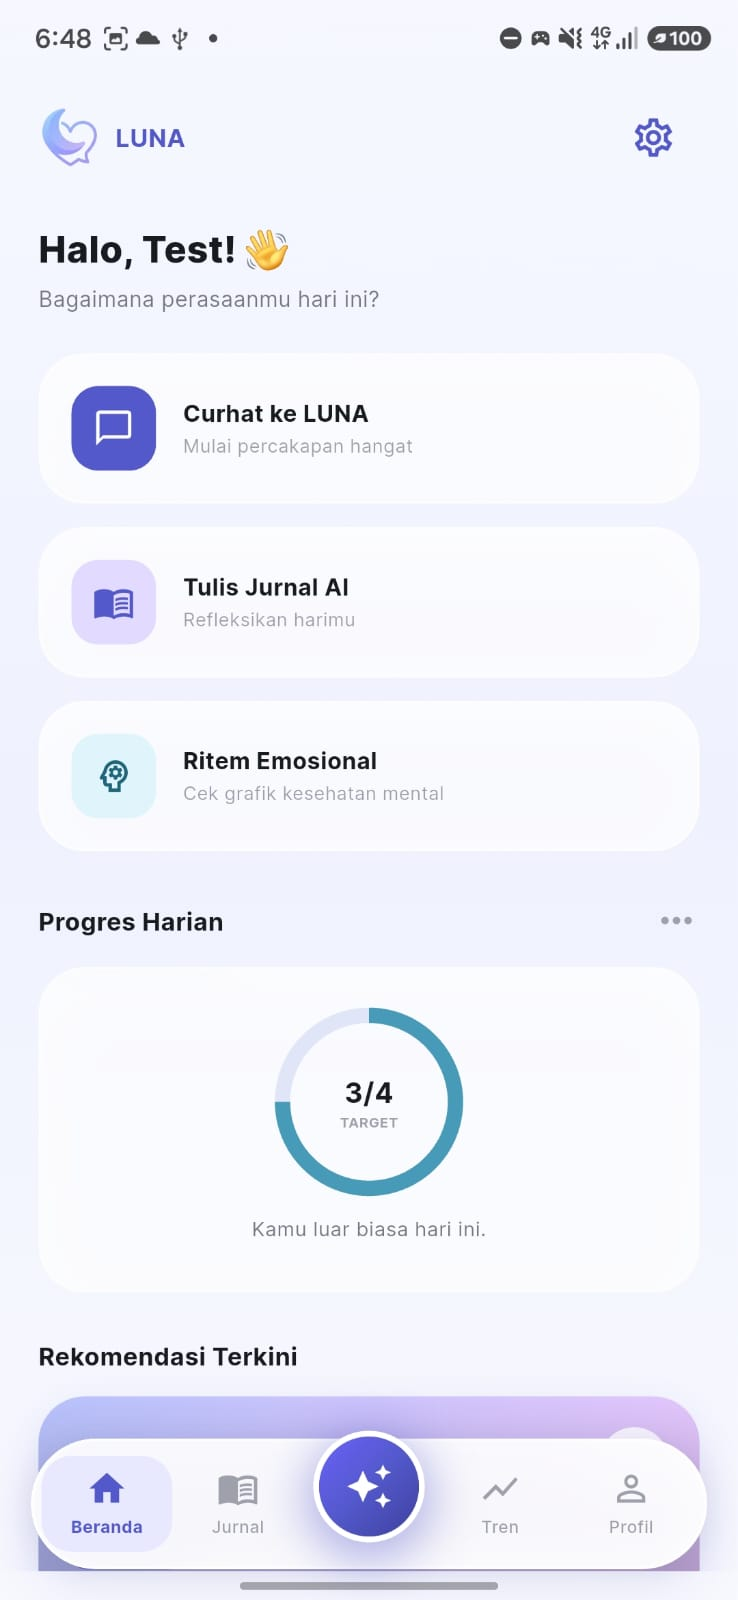
\includegraphics[height=5.8cm,keepaspectratio]{images/prototype/counseling_nav.jpeg}
            };
        \end{tikzpicture}\\[0.3em]
        {\small\itshape (a) Antarmuka Percakapan Teks}
    \end{minipage}%
    \hfill
    \begin{minipage}[b]{0.45\textwidth}
        \centering
        \begin{tikzpicture}
            \node[
                draw=TealAccent,
                fill=white,
                line width=0.8pt,
                rounded corners=6pt,
                inner sep=2pt
            ] {
                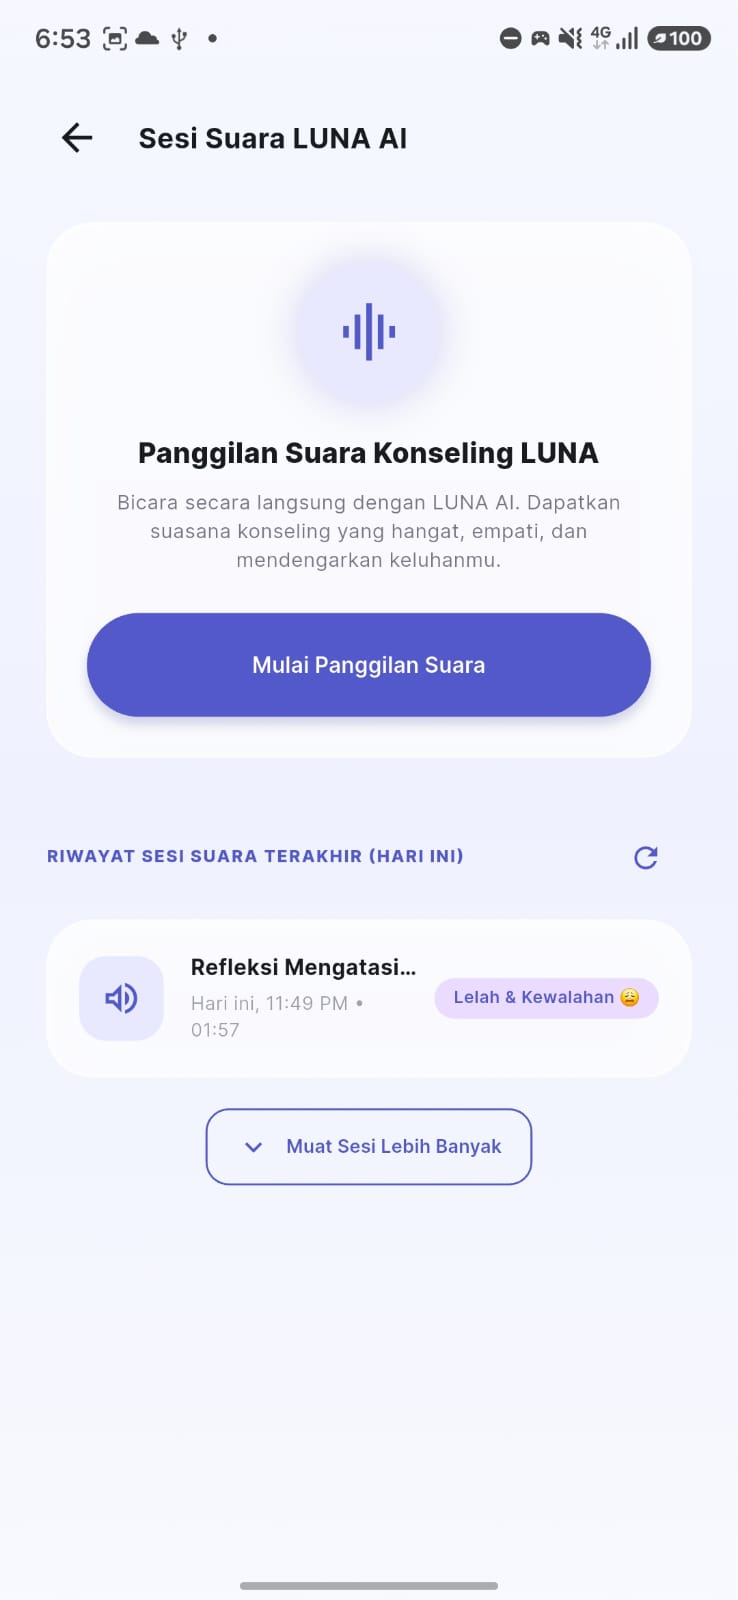
\includegraphics[height=5.8cm,keepaspectratio]{images/prototype/counseling_voice_entry.jpeg}
            };
        \end{tikzpicture}\\[0.3em]
        {\small\itshape (b) Penyiapan Sesi Suara}
    \end{minipage}
    \vspace{0.2em}
    \caption{AI Conversation}
\end{figure}

\subsubsecstyle{f. Voice Call}
\begin{figure}[H]
    \centering
    \begin{minipage}[b]{0.45\textwidth}
        \centering
        \begin{tikzpicture}
            \node[
                draw=TealAccent,
                fill=white,
                line width=0.8pt,
                rounded corners=6pt,
                inner sep=2pt
            ] {
                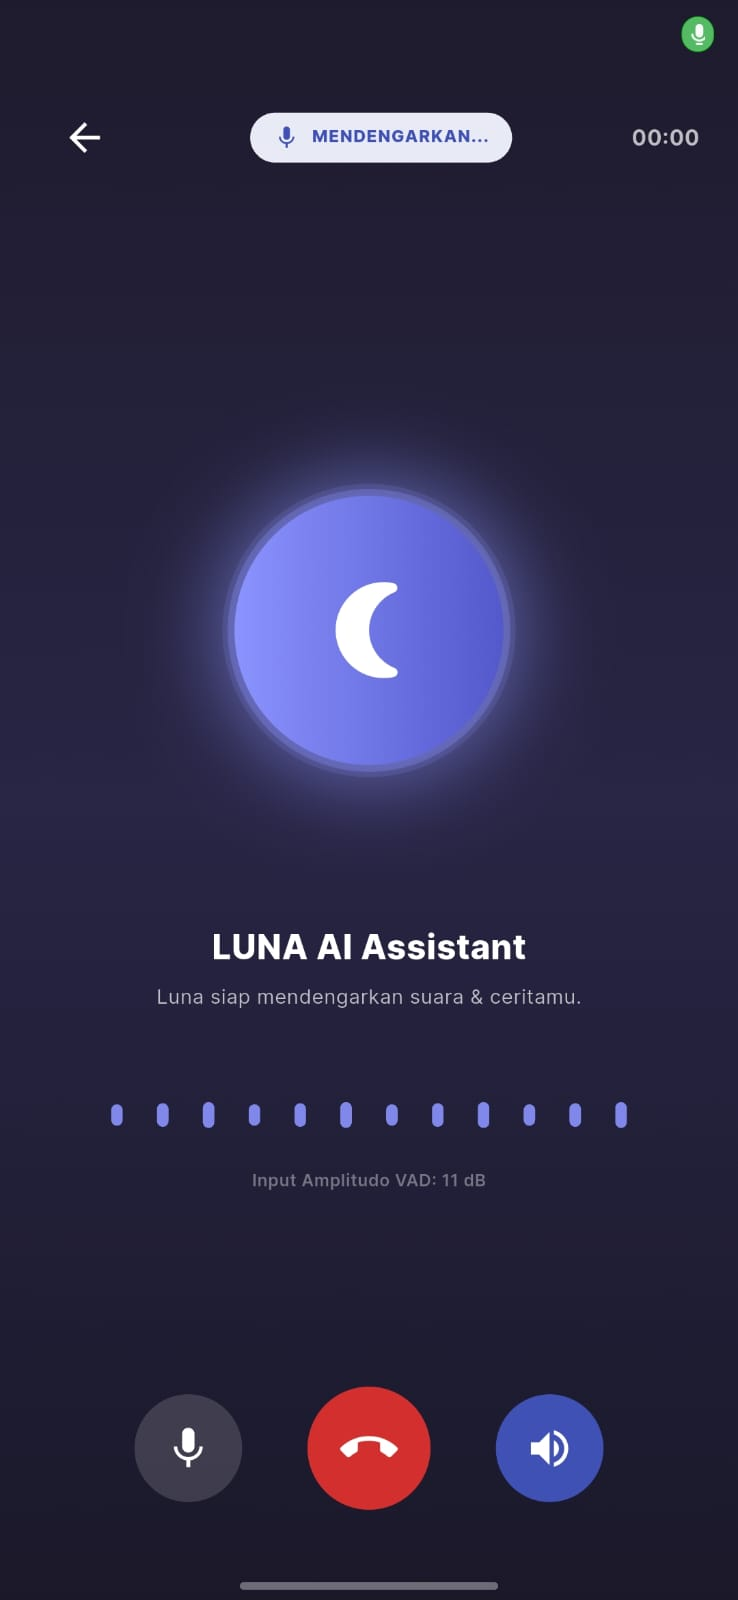
\includegraphics[height=5.8cm,keepaspectratio]{images/prototype/counseling_in_call.jpeg}
            };
        \end{tikzpicture}\\[0.3em]
        {\small\itshape (a) Panggilan Suara Real-Time Aktif}
    \end{minipage}%
    \hfill
    \begin{minipage}[b]{0.45\textwidth}
        \centering
        \begin{tikzpicture}
            \node[
                draw=TealAccent,
                fill=white,
                line width=0.8pt,
                rounded corners=6pt,
                inner sep=2pt
            ] {
                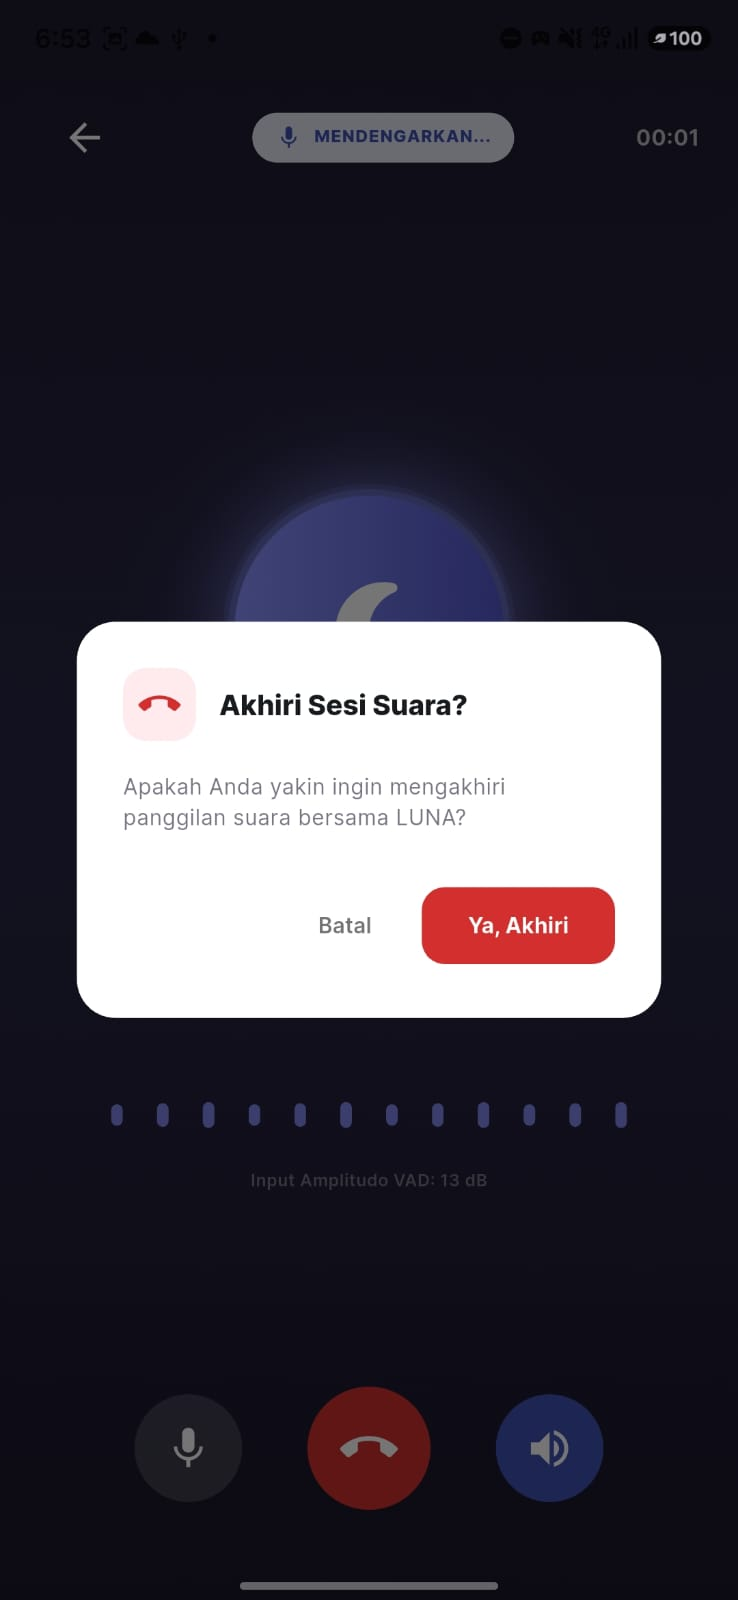
\includegraphics[height=5.8cm,keepaspectratio]{images/prototype/counseling_end_call.jpeg}
            };
        \end{tikzpicture}\\[0.3em]
        {\small\itshape (b) Kontrol \& Penghentian Panggilan}
    \end{minipage}
    \vspace{0.2em}
    \caption{Voice Call}
\end{figure}

\subsubsecstyle{g. AI Diary}
\begin{figure}[H]
    \centering
    \begin{minipage}[b]{0.45\textwidth}
        \centering
        \begin{tikzpicture}
            \node[
                draw=TealAccent,
                fill=white,
                line width=0.8pt,
                rounded corners=6pt,
                inner sep=2pt
            ] {
                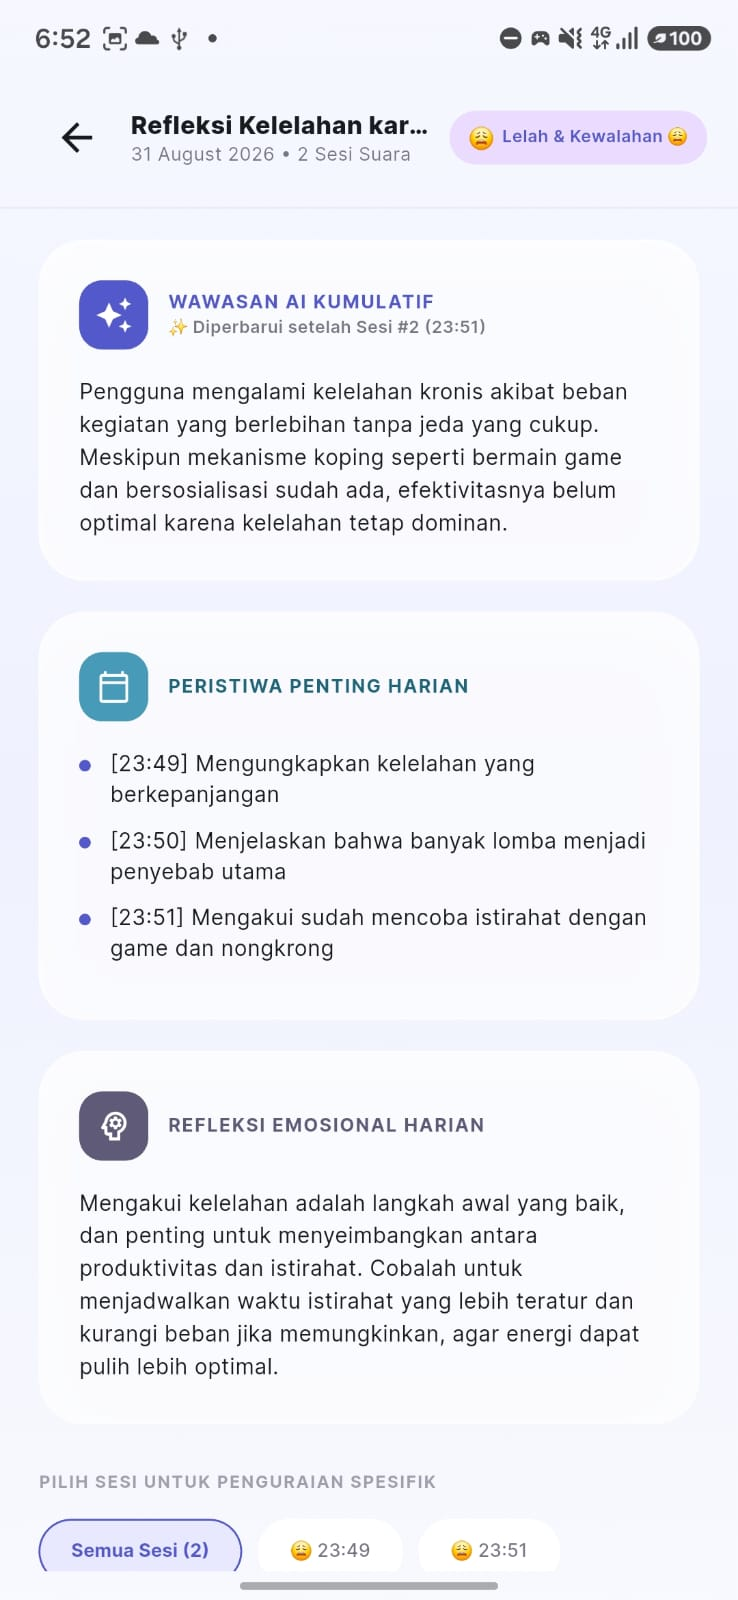
\includegraphics[height=5.8cm,keepaspectratio]{images/prototype/journal_page_1.jpeg}
            };
        \end{tikzpicture}\\[0.3em]
        {\small\itshape (a) Daftar Sintesis Jurnal Harian}
    \end{minipage}%
    \hfill
    \begin{minipage}[b]{0.45\textwidth}
        \centering
        \begin{tikzpicture}
            \node[
                draw=TealAccent,
                fill=white,
                line width=0.8pt,
                rounded corners=6pt,
                inner sep=2pt
            ] {
                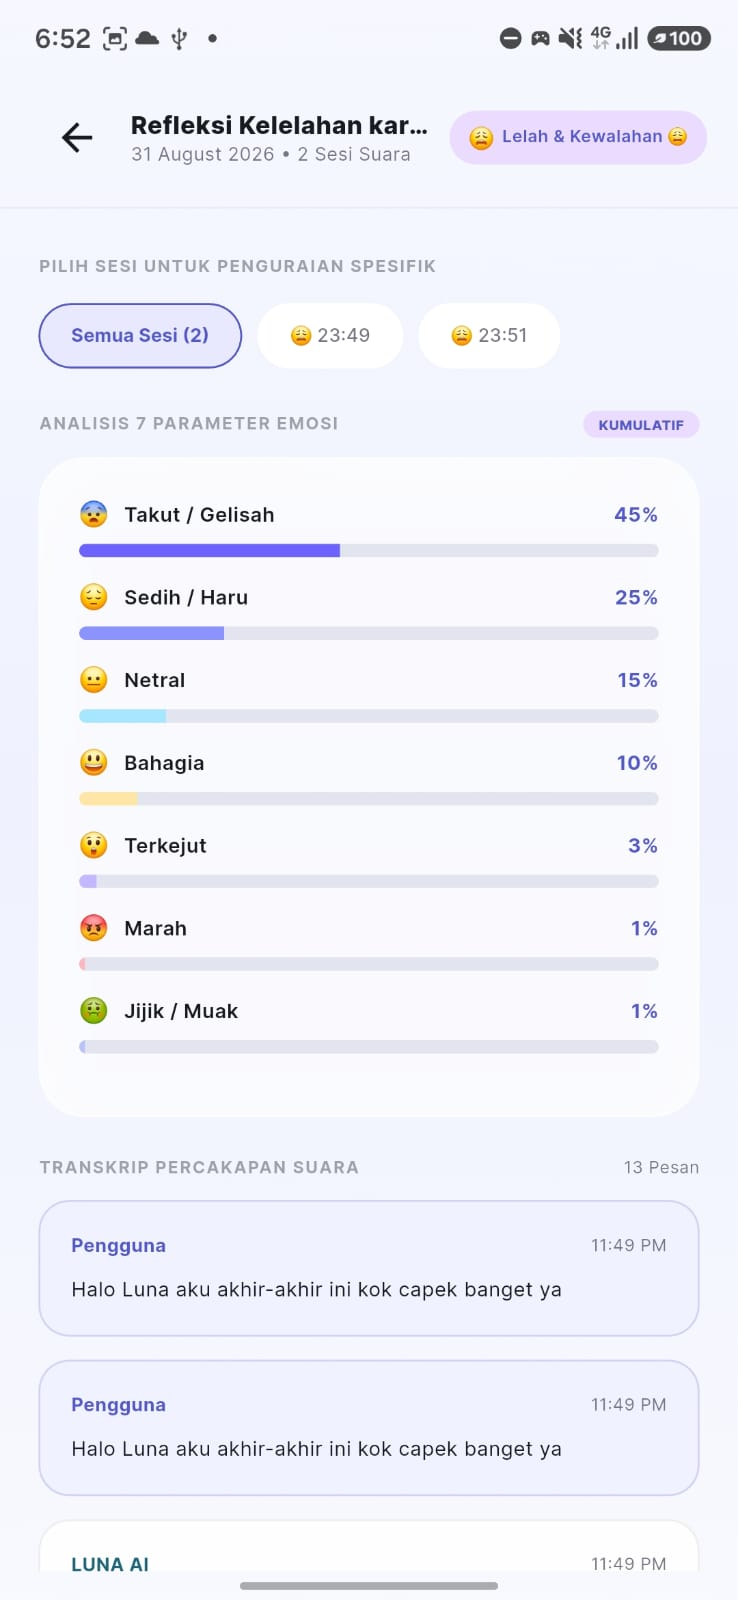
\includegraphics[height=5.8cm,keepaspectratio]{images/prototype/journal_page_2.jpeg}
            };
        \end{tikzpicture}\\[0.3em]
        {\small\itshape (b) Detail Analisis Jurnal Emosional}
    \end{minipage}
    \vspace{0.2em}
    \caption{AI Diary}
\end{figure}

\subsubsecstyle{h. Mental Health Monitoring}
\begin{figure}[H]
    \centering
    \begin{minipage}[b]{0.45\textwidth}
        \centering
        \begin{tikzpicture}
            \node[
                draw=TealAccent,
                fill=white,
                line width=0.8pt,
                rounded corners=6pt,
                inner sep=2pt
            ] {
                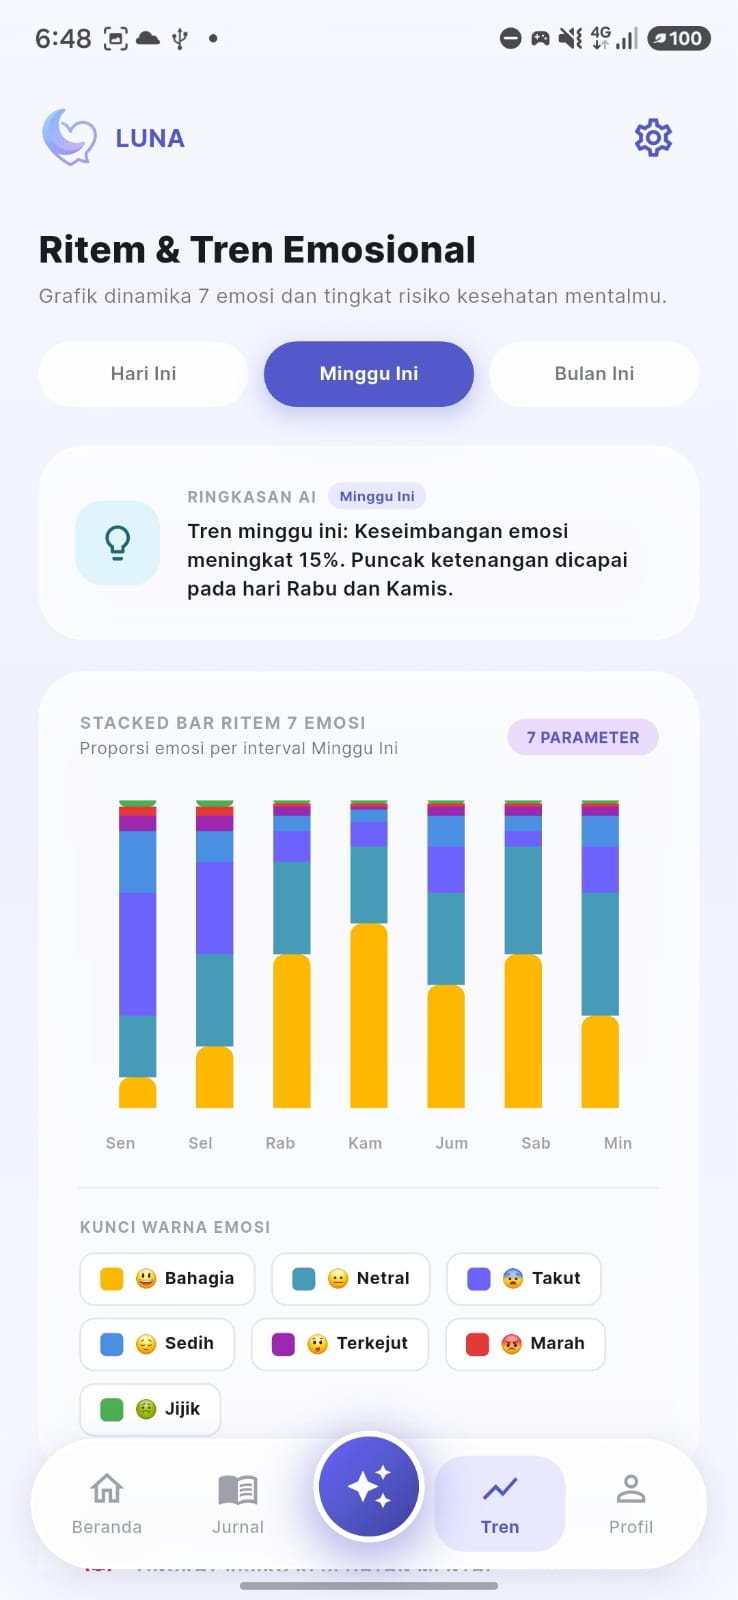
\includegraphics[height=5.8cm,keepaspectratio]{images/prototype/dashboard_page_1.jpeg}
            };
        \end{tikzpicture}\\[0.3em]
        {\small\itshape (a) Mood Tracker Harian}
    \end{minipage}%
    \hfill
    \begin{minipage}[b]{0.45\textwidth}
        \centering
        \begin{tikzpicture}
            \node[
                draw=TealAccent,
                fill=white,
                line width=0.8pt,
                rounded corners=6pt,
                inner sep=2pt
            ] {
                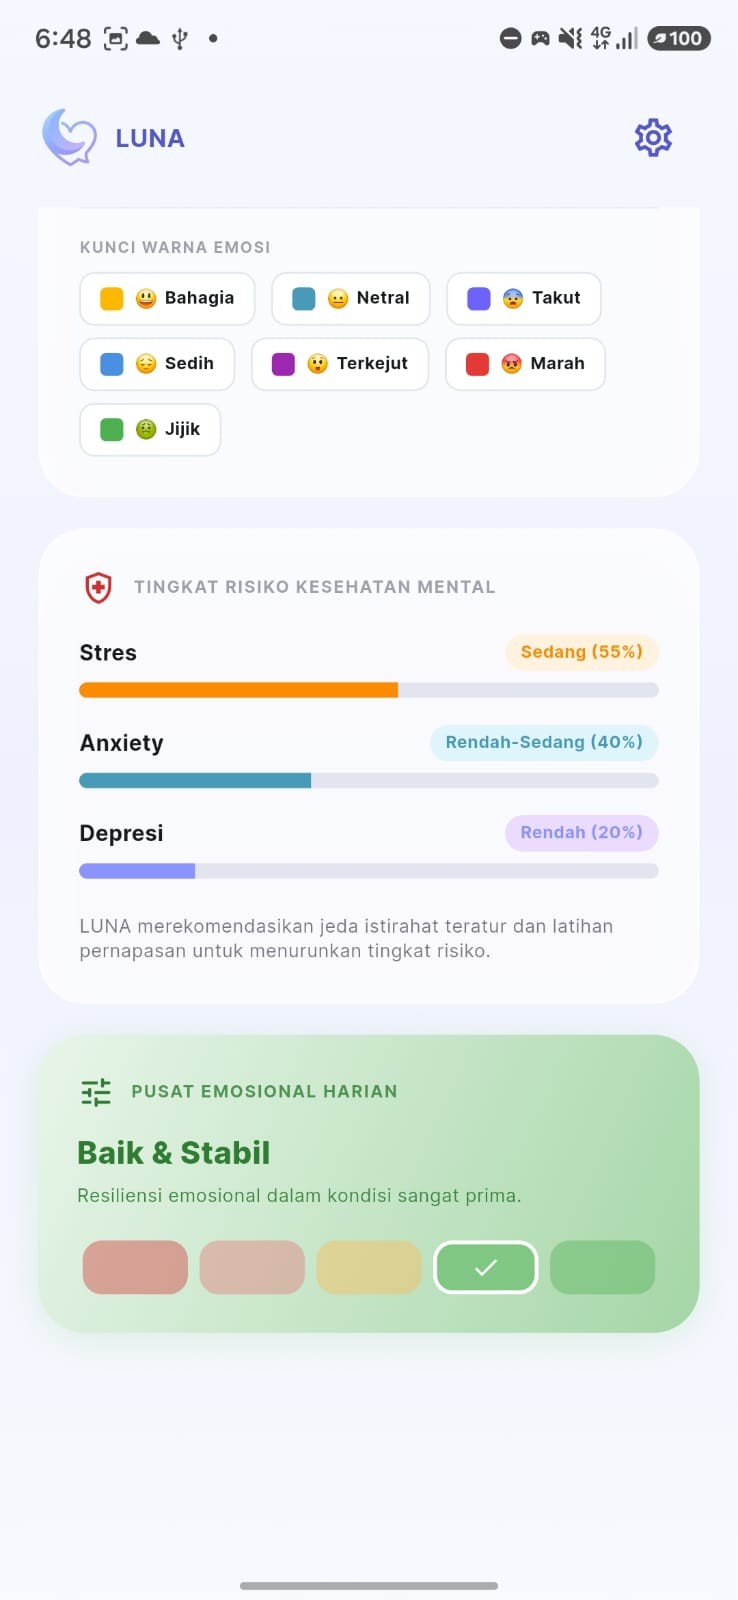
\includegraphics[height=5.8cm,keepaspectratio]{images/prototype/dashboard_page_2.jpeg}
            };
        \end{tikzpicture}\\[0.3em]
        {\small\itshape (b) Grafik Analisis Tren Emosional}
    \end{minipage}
    \vspace{0.2em}
    \caption{Mental Health Monitoring}
\end{figure}

\subsubsecstyle{i. Personalized Recommendation}
\begin{figure}[H]
    \centering
    \begin{minipage}[b]{0.45\textwidth}
        \centering
        \begin{tikzpicture}
            \node[
                draw=TealAccent,
                fill=white,
                line width=0.8pt,
                rounded corners=6pt,
                inner sep=2pt
            ] {
                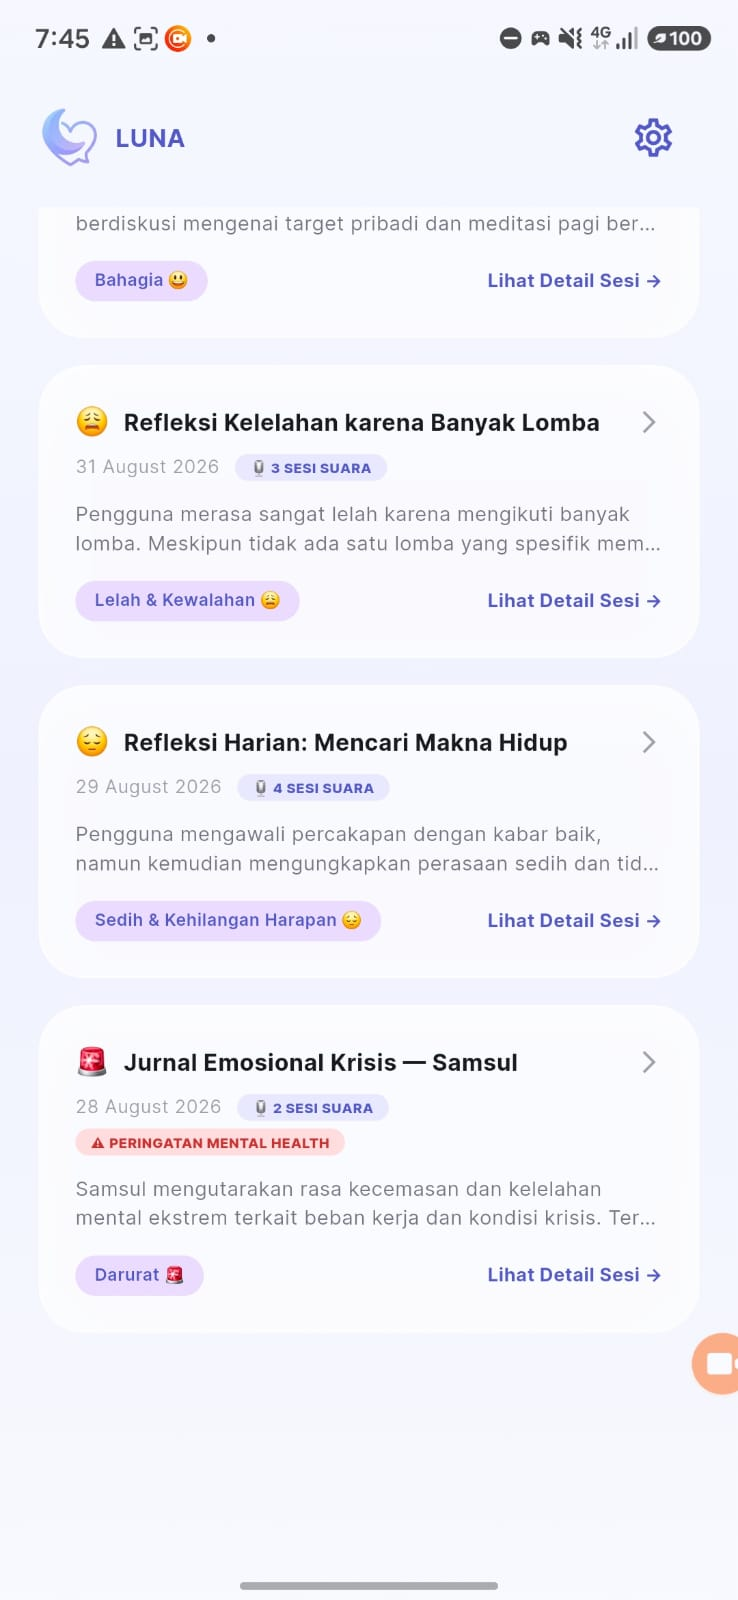
\includegraphics[height=5.8cm,keepaspectratio]{images/prototype/journal_list_crisis.jpeg}
            };
        \end{tikzpicture}\\[0.3em]
        {\small\itshape (a) Daftar Jurnal Risiko Tinggi}
    \end{minipage}%
    \hfill
    \begin{minipage}[b]{0.45\textwidth}
        \centering
        \begin{tikzpicture}
            \node[
                draw=TealAccent,
                fill=white,
                line width=0.8pt,
                rounded corners=6pt,
                inner sep=2pt
            ] {
                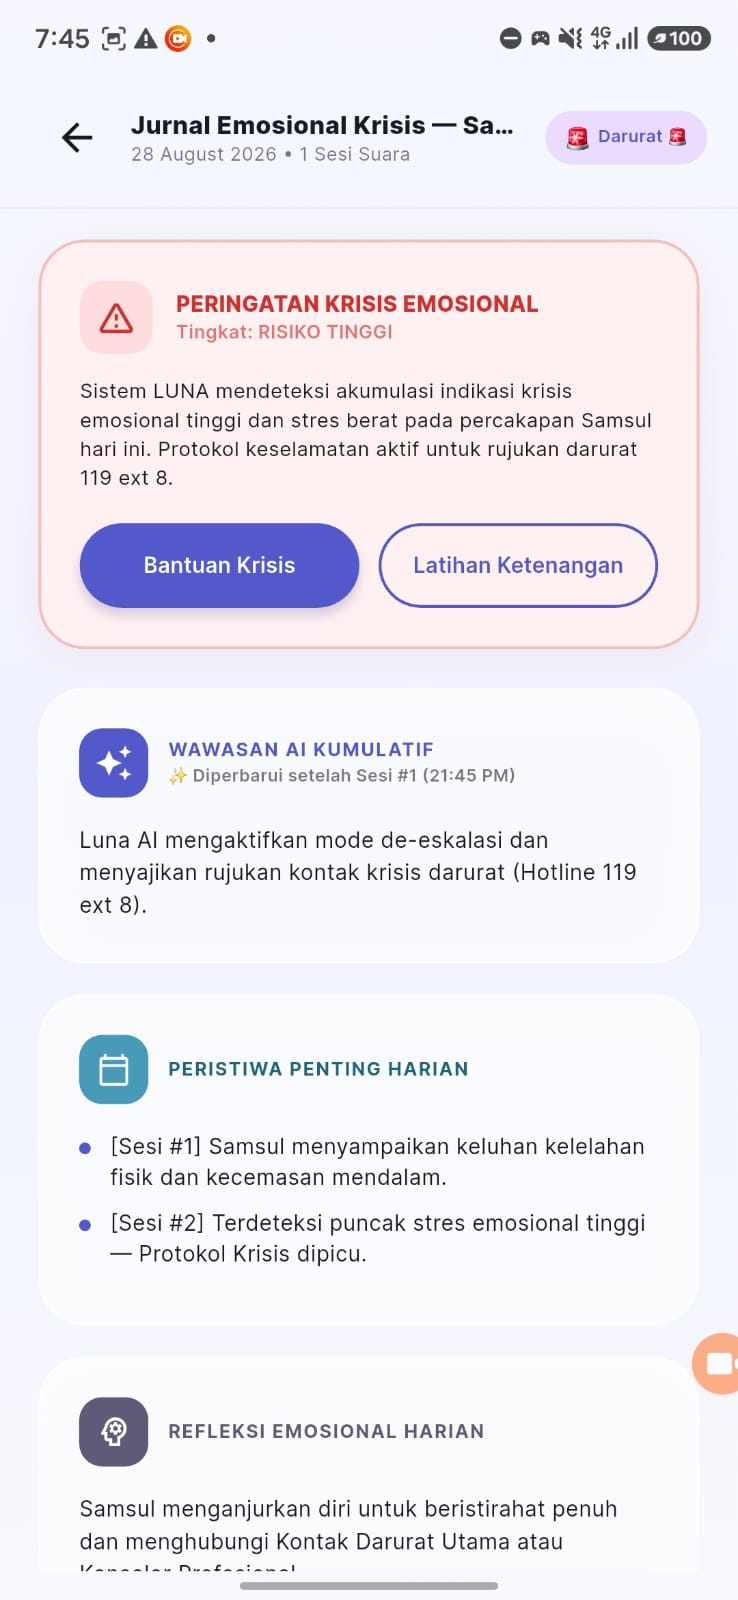
\includegraphics[height=5.8cm,keepaspectratio]{images/prototype/journal_detail_crisis.jpeg}
            };
        \end{tikzpicture}\\[0.3em]
        {\small\itshape (b) Detail Rekomendasi \& Intervensi}
    \end{minipage}
    \vspace{0.2em}
    \caption{Personalized Recommendation}
\end{figure}

\subsubsecstyle{j. Support \& Emergency}
\begin{figure}[H]
    \centering
    \begin{minipage}[b]{0.45\textwidth}
        \centering
        \begin{tikzpicture}
            \node[
                draw=TealAccent,
                fill=white,
                line width=0.8pt,
                rounded corners=6pt,
                inner sep=2pt
            ] {
                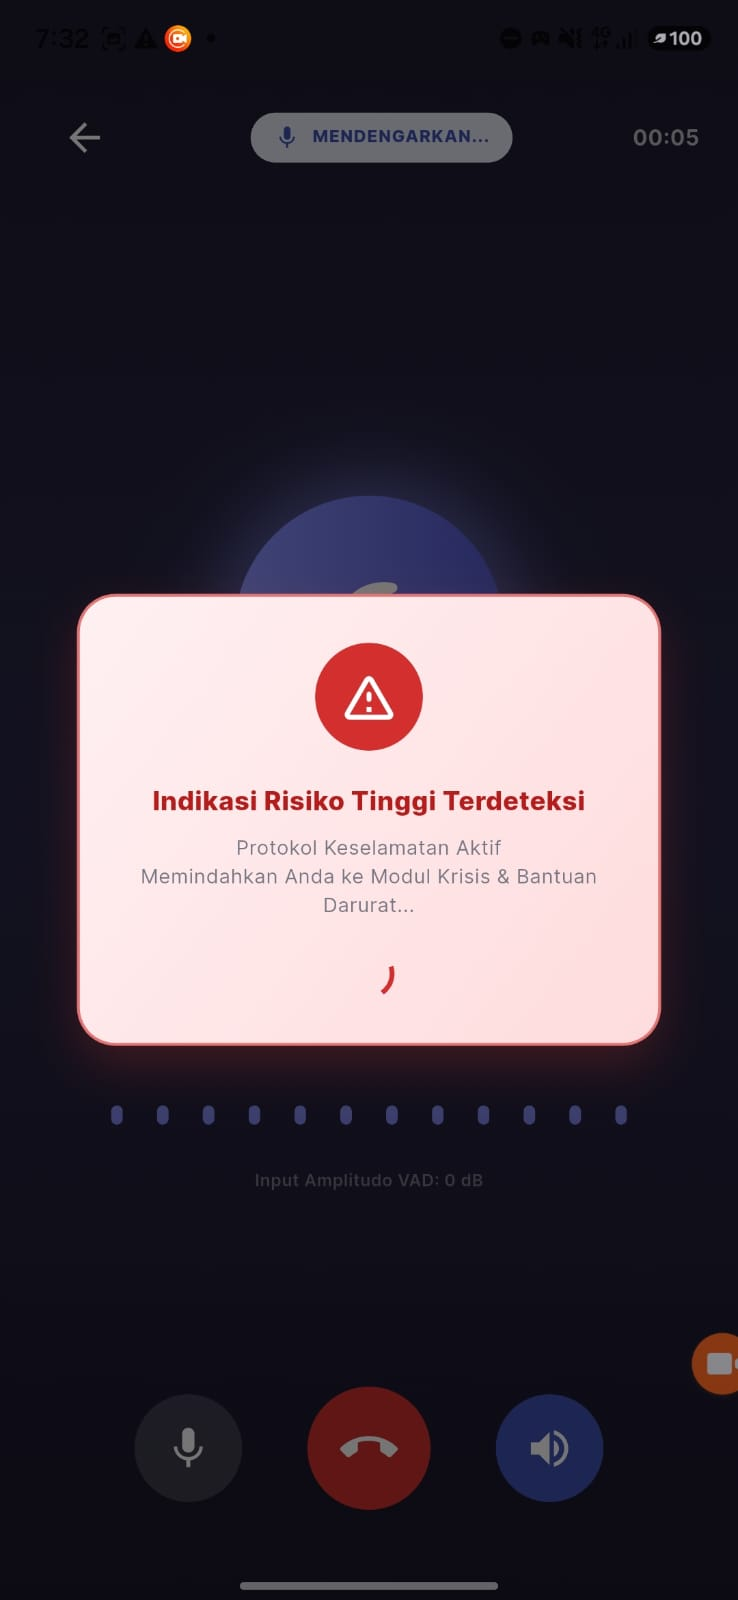
\includegraphics[height=5.8cm,keepaspectratio]{images/prototype/crisis_alert_dialog.jpeg}
            };
        \end{tikzpicture}\\[0.3em]
        {\small\itshape (a) Pop-up Peringatan High Risk}
    \end{minipage}%
    \hfill
    \begin{minipage}[b]{0.45\textwidth}
        \centering
        \begin{tikzpicture}
            \node[
                draw=TealAccent,
                fill=white,
                line width=0.8pt,
                rounded corners=6pt,
                inner sep=2pt
            ] {
                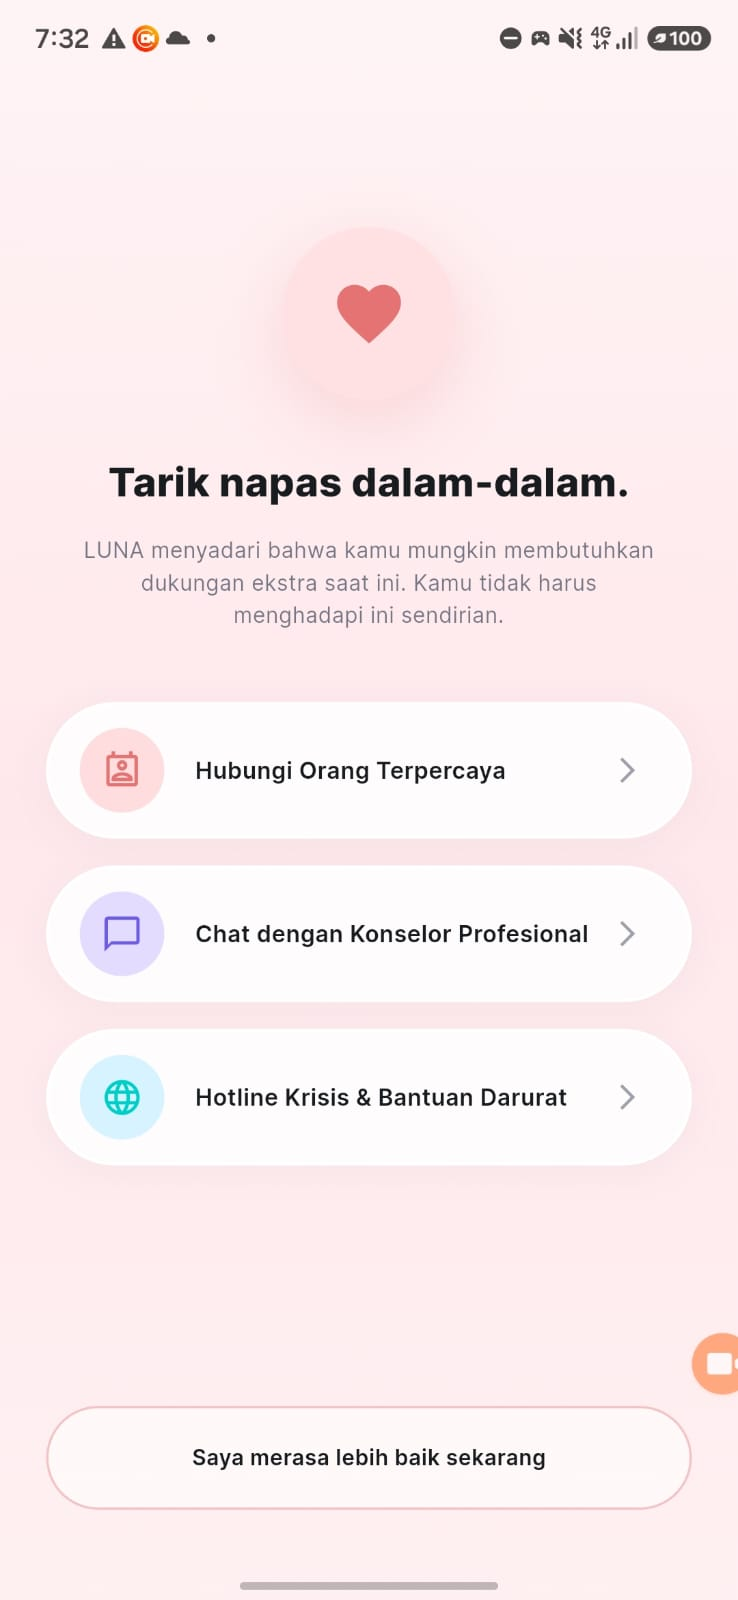
\includegraphics[height=5.8cm,keepaspectratio]{images/prototype/crisis_module_screen.jpeg}
            };
        \end{tikzpicture}\\[0.3em]
        {\small\itshape (b) Layar Modul Krisis \& Support Hotline}
    \end{minipage}
    \vspace{0.2em}
    \caption{Support \& Emergency}
\end{figure}

\clearpage
\lampiranhead{5. Dokumentasi Penggunaan}

\subsubsecstyle{a. Membuka Aplikasi}
\noindent\textbf{Tujuan:} Masuk ke halaman utama LUNA (Gambar 9, 10).\par
\noindent\textbf{Langkah:}
\begin{enumerate}[leftmargin=1.5em,label=\arabic*.,itemsep=2pt,topsep=2pt]
    \item Buka aplikasi LUNA.
    \item Pilih Login atau Daftar.
    \item Masuk ke Home.
\end{enumerate}

\subsubsecstyle{b. Memulai Percakapan AI}
\noindent\textbf{Tujuan:} Memulai sesi konsultasi (Gambar 13).\par
\noindent\textbf{Langkah:}
\begin{enumerate}[leftmargin=1.5em,label=\arabic*.,itemsep=2pt,topsep=2pt]
    \item Tekan menu AI Conversation.
    \item Ketik pesan atau gunakan mikrofon.
    \item AI mulai merespons.
\end{enumerate}

\subsubsecstyle{c. Voice Conversation}
\noindent\textbf{Tujuan:} Melakukan percakapan suara (Gambar 14).\par
\noindent\textbf{Langkah:}
\begin{enumerate}[leftmargin=1.5em,label=\arabic*.,itemsep=2pt,topsep=2pt]
    \item Tekan tombol Voice.
    \item Izinkan akses mikrofon.
    \item Mulai berbicara.
    \item AI memberikan respons suara.
\end{enumerate}

\subsubsecstyle{d. AI Diary}
\noindent\textbf{Tujuan:} Melihat diary otomatis (Gambar 15).\par
\noindent\textbf{Langkah:}
\begin{enumerate}[leftmargin=1.5em,label=\arabic*.,itemsep=2pt,topsep=2pt]
    \item Buka menu Diary.
    \item Pilih tanggal.
    \item Sistem menampilkan ringkasan percakapan.
\end{enumerate}

\subsubsecstyle{e. Monitoring}
\noindent\textbf{Tujuan:} Melihat perkembangan kondisi mental (Gambar 16).\par
\noindent\textbf{Langkah:}
\begin{enumerate}[leftmargin=1.5em,label=\arabic*.,itemsep=2pt,topsep=2pt]
    \item Pilih menu Monitoring.
    \item Sistem menampilkan grafik emosi.
    \item Lihat perubahan kondisi dari waktu ke waktu.
\end{enumerate}

\subsubsecstyle{f. Recommendation}
\noindent\textbf{Tujuan:} Melihat rekomendasi personal (Gambar 17).\par
\noindent\textbf{Langkah:}
\begin{enumerate}[leftmargin=1.5em,label=\arabic*.,itemsep=2pt,topsep=2pt]
    \item Buka Recommendation.
    \item Sistem menampilkan aktivitas yang direkomendasikan.
    \item Pengguna dapat menandai aktivitas sebagai selesai.
\end{enumerate}

\subsubsecstyle{g. Support}
\noindent\textbf{Tujuan:} Mengakses bantuan ketika diperlukan (Gambar 18).\par
\noindent\textbf{Langkah:}
\begin{enumerate}[leftmargin=1.5em,label=\arabic*.,itemsep=2pt,topsep=2pt]
    \item Pilih menu Support.
    \item Sistem menampilkan informasi bantuan.
    \item Jika diperlukan, sistem memberikan arahan sesuai tingkat risiko.
\end{enumerate}

\clearpage
\lampiranhead{6. Bukti Wawancara Psikolog (Studi Pendahuluan DASS-21 \& Rencana Uji Coba)}

\indent Dokumentasi wawancara klinis dan konsultasi ilmiah bersama \textbf{Qori Fanani, M.Psi., Psikolog} (Petugas Poliklinik Politeknik Negeri Malang dan Dosen Psikologi Universitas Kepanjen) mengenai validasi kerangka kerja instrumen DASS-21 (\textit{Depression Anxiety Stress Scale 21}) serta penjajakan kerja sama \textit{clinical trial} aplikasi LUNA disajikan pada Gambar 19.

\indent Melalui diskusi ini, pakar mengonfirmasi validitas pembagian tingkat keparahan distres mental pengguna menjadi Level 1 (\textit{Mild}), Level 2 (\textit{Moderate}), dan Level 3 (\textit{Severe/Extremely Severe}) yang diterapkan pada mesin pemicu intervensi LUNA. Selain itu, pihak Poliklinik Polinema menyambut baik dan sangat terbuka terhadap pelaksanaan \textit{pilot testing} dan uji coba klinis penggunaan LUNA pada mahasiswa maupun pasien Poliklinik Polinema sebagai bagian dari peta jalan evaluasi efektivitas sistem.

\begin{figure}[H]
    \centering
    \begin{tikzpicture}
        \node[
            draw=TealAccent,
            fill=white,
            line width=0.8pt,
            rounded corners=6pt,
            inner sep=2pt
        ] {
            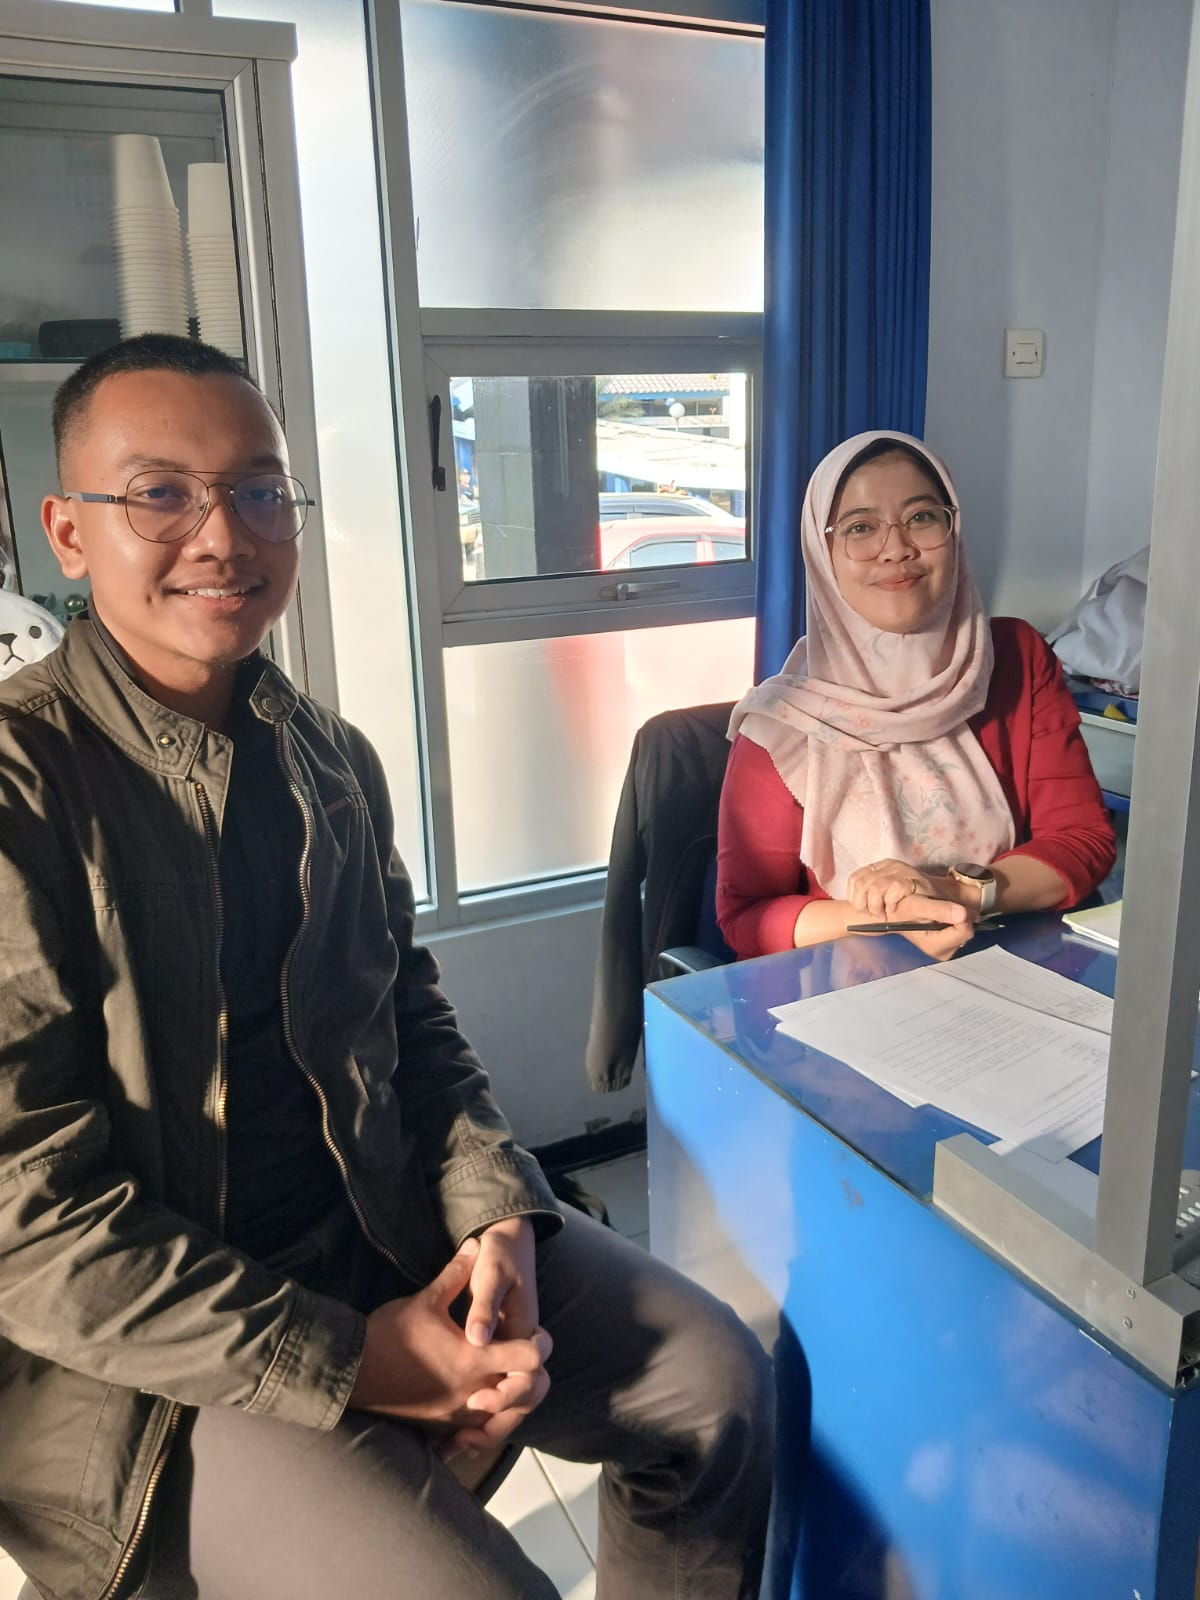
\includegraphics[height=12.5cm,keepaspectratio]{images/lampiran/fig9_wawancara_psikolog.png}
        };
    \end{tikzpicture}
    \caption{Dokumentasi Wawancara dengan Qori Fanani, M.Psi., Psikolog}
\end{figure}

\clearpage
\lampiranhead{7. Surat Pernyataan Orisinalitas Karya}

\begin{figure}[H]
    \centering
    \begin{tikzpicture}
        \node[
            draw=TealAccent,
            fill=white,
            line width=0.8pt,
            rounded corners=6pt,
            inner sep=2pt
        ] {
            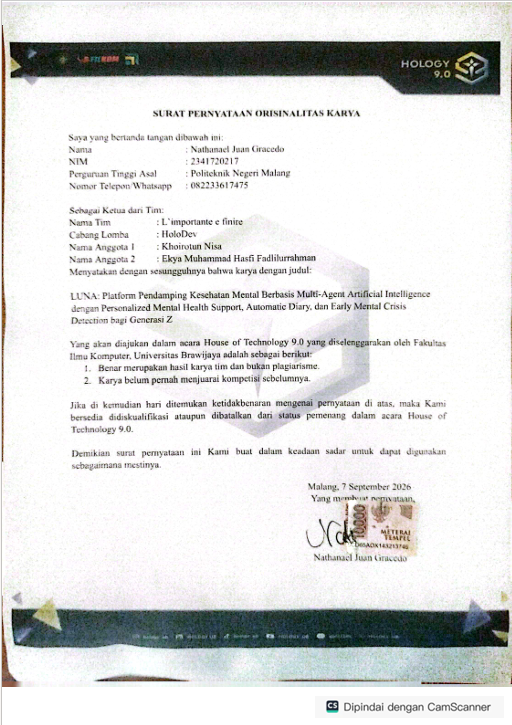
\includegraphics[width=0.88\textwidth,keepaspectratio]{images/surat pernyataan.png}
        };
    \end{tikzpicture}
    \caption{Surat Pernyataan Orisinalitas Karya (Ber-meterai \& Ditandatangani)}
\end{figure}

\clearpage
\lampiranhead{8. Tautan Video Demo Aplikasi \& Berkas Akses}

\indent Sebagai pemenuhan persyaratan kompetisi HoloDev HOLOGY 9.0, berikut adalah daftar tautan akses publik untuk video pengujian demo perangkat lunak dan repositori berkas implementasi:

\begin{enumerate}[leftmargin=*,label=\arabic*.,itemsep=0.5em]
    \item \textbf{Tautan Video Demo Aplikasi (Google Drive):}\\
    \url{https://drive.google.com/file/d/1leySp4r29Kz3TLDlhNC1YP4iOxChis1a/view?usp=drive_link}\\
    {\small\itshape (Video berdurasi $\le$ 10 menit berisi pengenalan tim, latar belakang solusi, serta peragaan fungsionalitas utama aplikasi LUNA).}
    
    \item \textbf{Tautan Google Drive Berkas Source Code, Build APK \& Dokumentasi:}\\
    \url{https://drive.google.com/drive/folders/1bJp6CdtFBXfh3RJ8tv2wlBQT3z1xdhio?usp=drive_link}\\
    {\small\itshape (Berisi berkas build APK/Web, source code backend FastAPI, FastMCP tools, dan kode aplikasi Flutter luna\_mobile).}
\end{enumerate}

